\chapter{Supplementary Results}
\label{app:A}

This appendix includes results that were redundant or not directly relevent to the discussions in the chapters.  They are provided here as supplementary and complimentary information.

\section{2D Scattering on Fermi}

Figure \ref{prelim_speedup_old} shows the speedup factors, $F_s=t_\mathrm{CPU}/t_\mathrm{GPU}$, of the GPU implementations discussed in Section \ref{sec:prelim}.  This benchmark was run on the same server with a 8-core AMD Opteron 6128 CPU clocked at 2.0GHz, but on a Tesla C2075 card.   The task-parallel implementation performs best, with a maximum speedup of around 29x.  The remapping implementation has the next best performance, with about a 20x speedup over the CPU. The batched implementation's performance departs from the remapping implementation at $10^5$ particles and even starts to deteriorate between $10^6$ and $10^7$ particles.  This is due to the transport having to be done in batches at this point due to the maximum block number of 65,536.  

\begin{figure}[h!] 
  \centering
    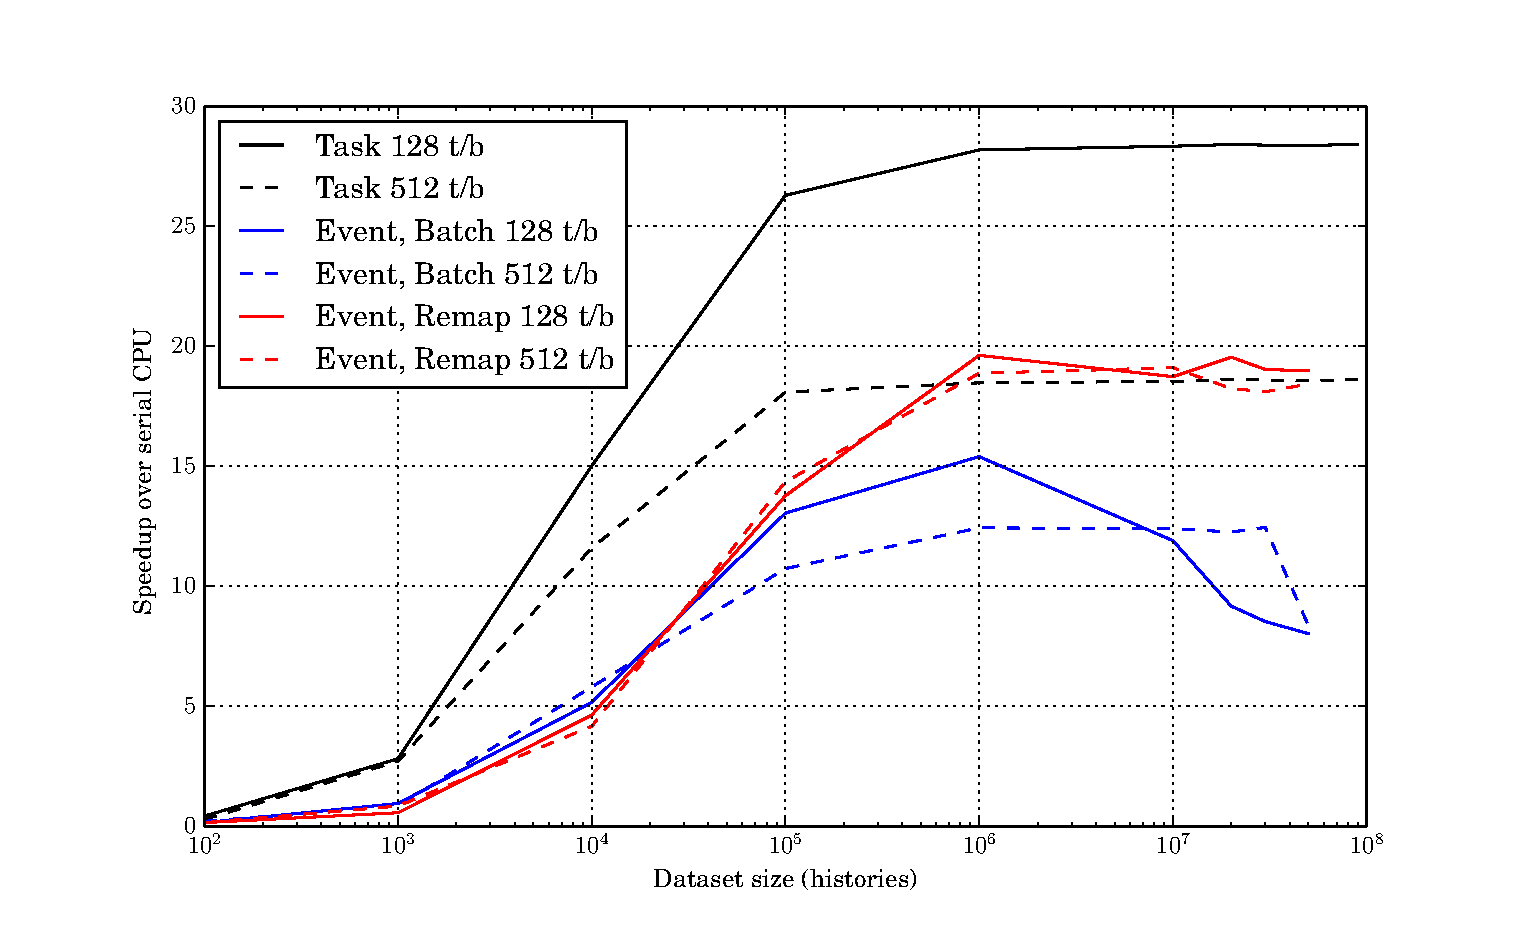
\includegraphics[width=0.8\textwidth]{graphics/prelim_speedup_old.eps}
     \caption{Speedup factors of the GPU implementations over the CPU implementation on a Tesla C2075. \label{prelim_speedup_old} }
\end{figure}

These results are quite different than those shown in Section \ref{sec:prelim} where the remapping version was decidedly faster than the others at large particle numbers.  The C2075 card is a Fermi architecture card, and has slightly different memory characteristics that the newer K20, which is a Kepler architecture card.  The likely reason that the older architecture is faster for these applications is that an important change was made in Kepler regarding the L1 cache.  The L1 cache was introduced in Fermi, and sits closest to the registers and processing units on the SMs.  ``Devices of compute capability 2.x come with an L1/L2 cache hierarchy that is used to cache local and global memory accesses \cite{fermi}.''    In Fermi, the L1 cache acts like a traditional CPU L1 and buffers access to the L2, which in turn buffers access to global memory.  In these simple applications, all particle data is access in global memory, but checks the L1 first.  A cache hit would increase access rate considerably, and since the history-based version keeps the same particle data in it (or registers) for its entire lifetime, and the particle does not carry much data, it most likely lives in L1 for the entire life of the particle.  In the event-based versions, multiple kernels are launched for every operation, and the caches are cleared in between launches.  This means that the particle data is fetched from global memory every time instead of being loaded from much faster L1.  This may also explain why the task-based performance drops to that of the remapping version when the threads per block is increased from 128 to 512.  The additional pressure on the registers causes the data to spill into L2 and the benefits of L1 caching (or always keeping the data in registers) are lost.

In Kepler, the L1 is reserved for register spills and local data access.  ``L1 caching in Kepler GPUs is reserved only for local memory accesses, such as register spills and stack data. Global loads are cached in L2 only (or in the Read-Only Data Cache) \cite{kepler}.''  This means that on Kepler, the task-based version does not benefit as much from from L1 cache hits as it did on Fermi, and must go to L2 or global memory every time particles data is loaded or spilled from registers.

The remapping version performs better than the non-remapping version for the very same reasons the remming version of WARP performs better than the non-remapping version.  Remapping creates more efficient, if non-coalesced, data access.  Since the amount of data required per neutron is greater in WARP than that of the particles in this preliminary study, the L1 cache would most likely be overflown anyway, and the remapping algorithm would be the best performing on Fermi as well as Kepler architectures.

\section{Serpent Fission Source Distributions}

\begin{figure}[h!] 
  \centering
    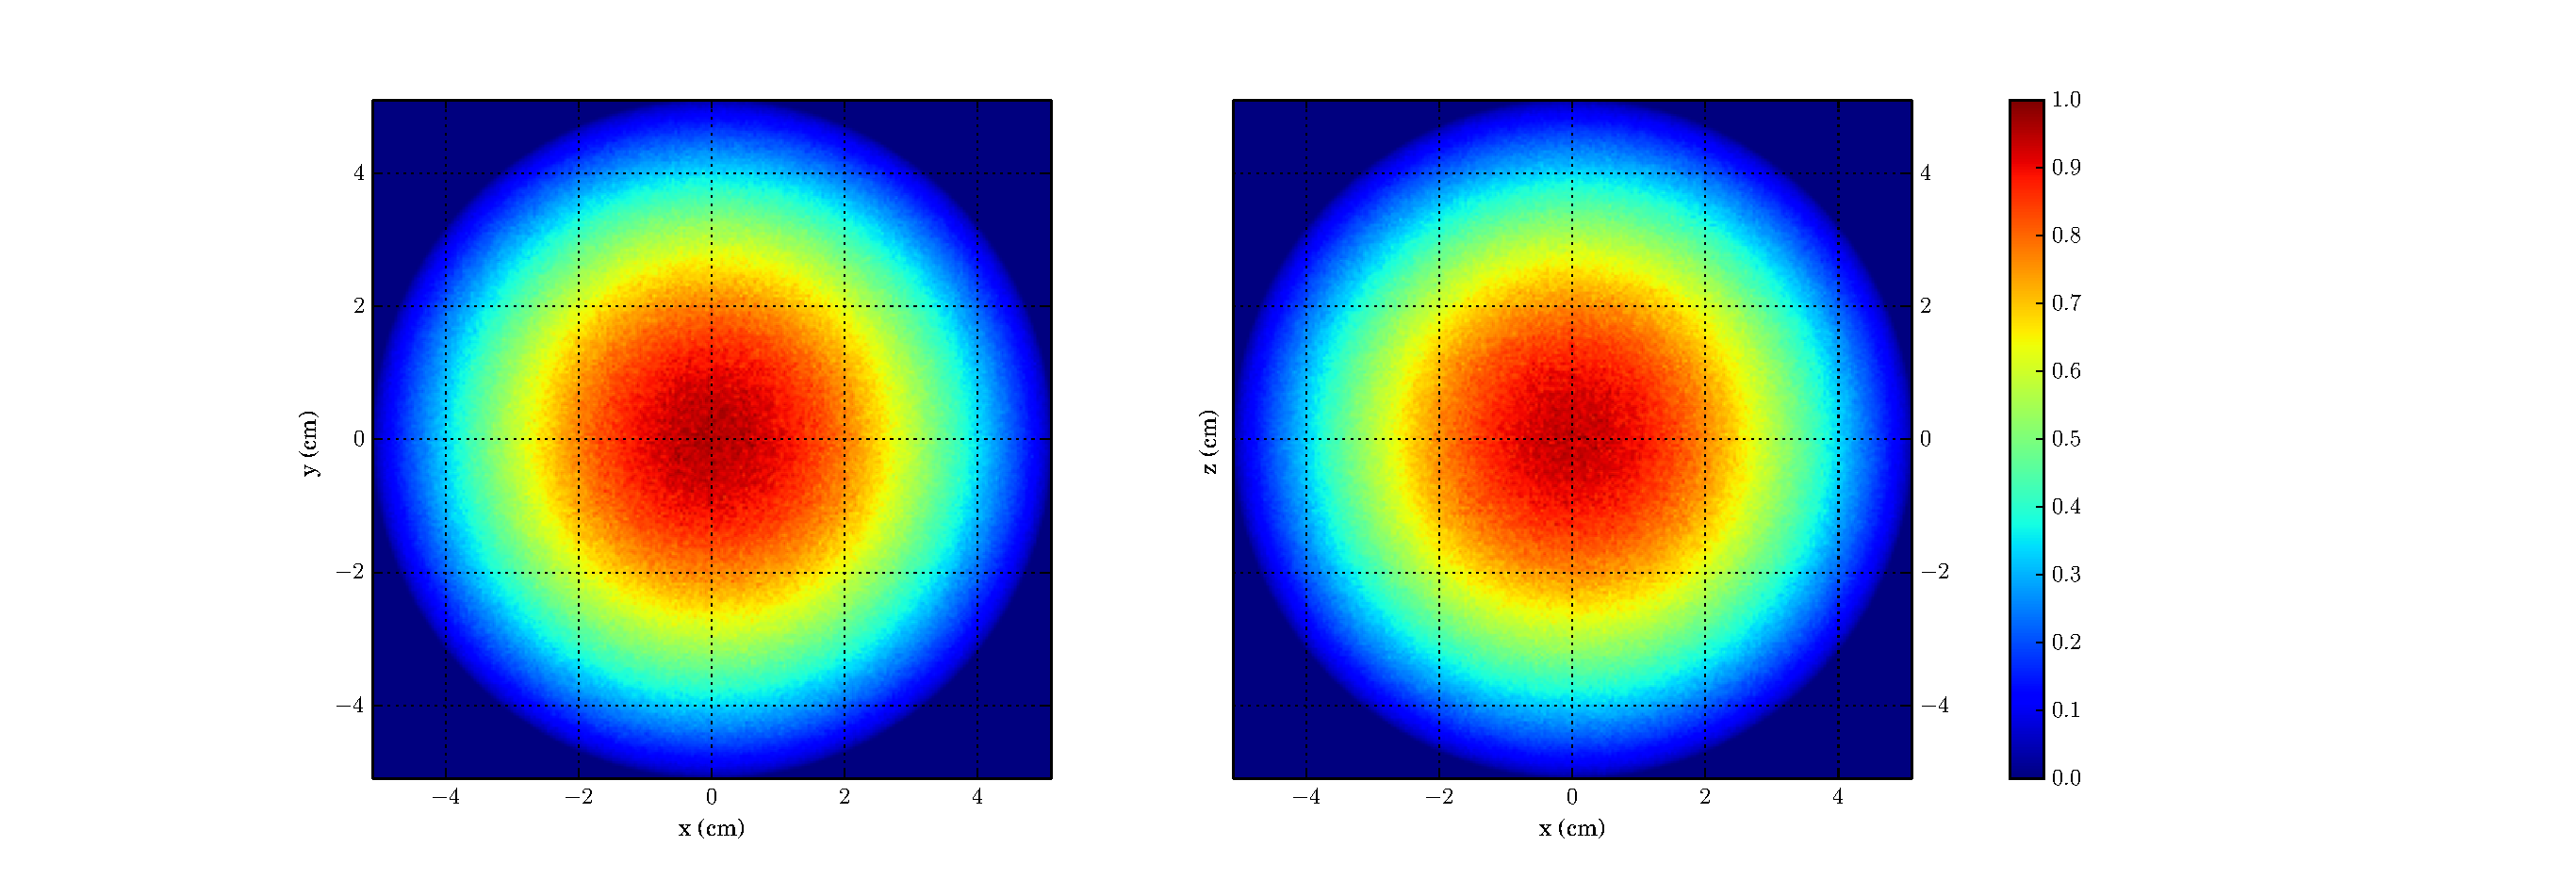
\includegraphics[width=\textwidth,trim= 4cm 0cm 6cm 0cm]{graphics/finalresults/godiva_fiss_serp-6.eps}
     \caption{Fission source distribution from Serpent 2.1.18 of a ``Jezebel'' bare Pu-239 sphere. \label{serp_godiva_mesh} }
\end{figure}

\begin{figure}[h!] 
  \centering
    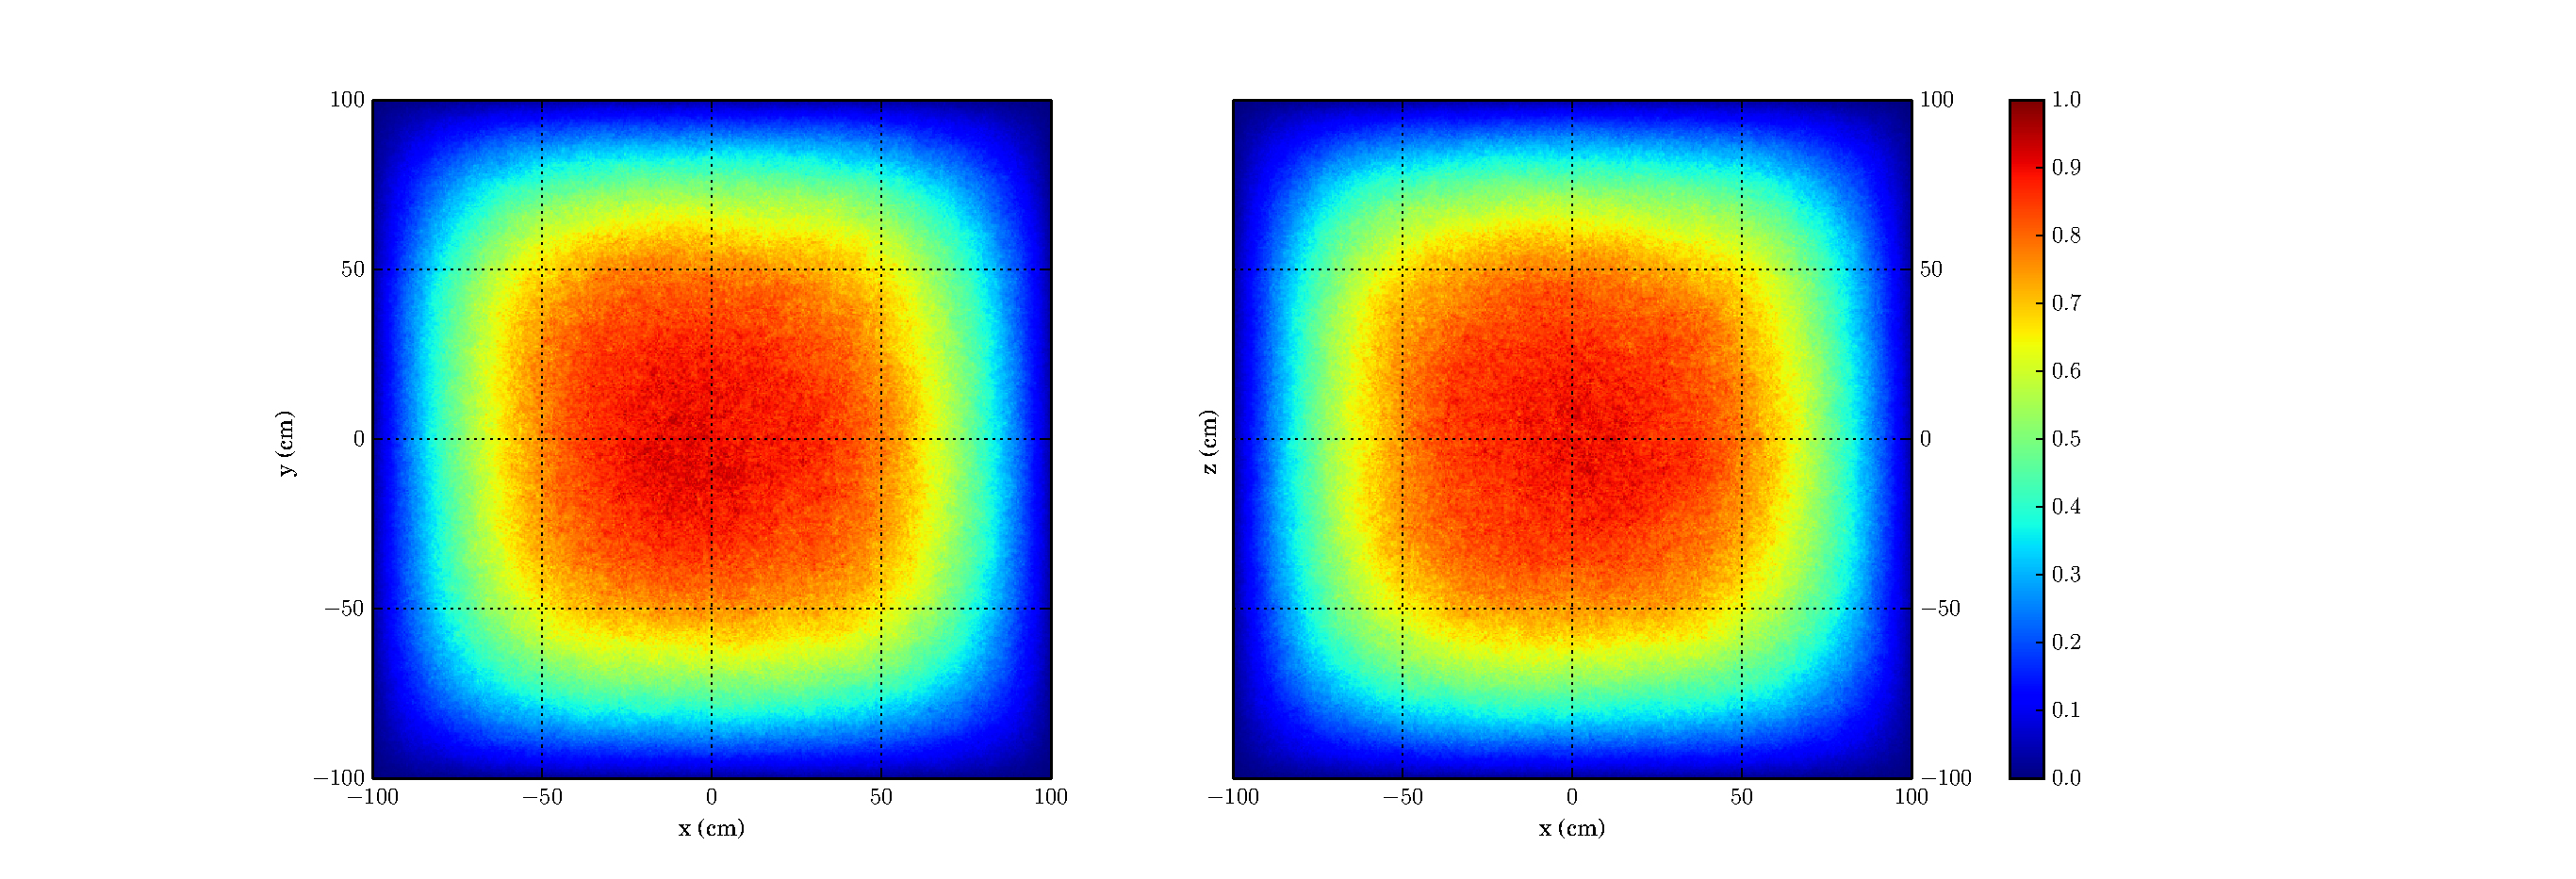
\includegraphics[width=\textwidth,trim= 4cm 0cm 6cm 0cm]{graphics/finalresults/homfuel_fiss_serp-6.eps}
     \caption{Fission source distribution from Serpent 2.1.18 of a homogenized block of UO$_2$ and water. \label{serp_homfuel_mesh} }
\end{figure}

\begin{figure}[h!] 
  \centering
    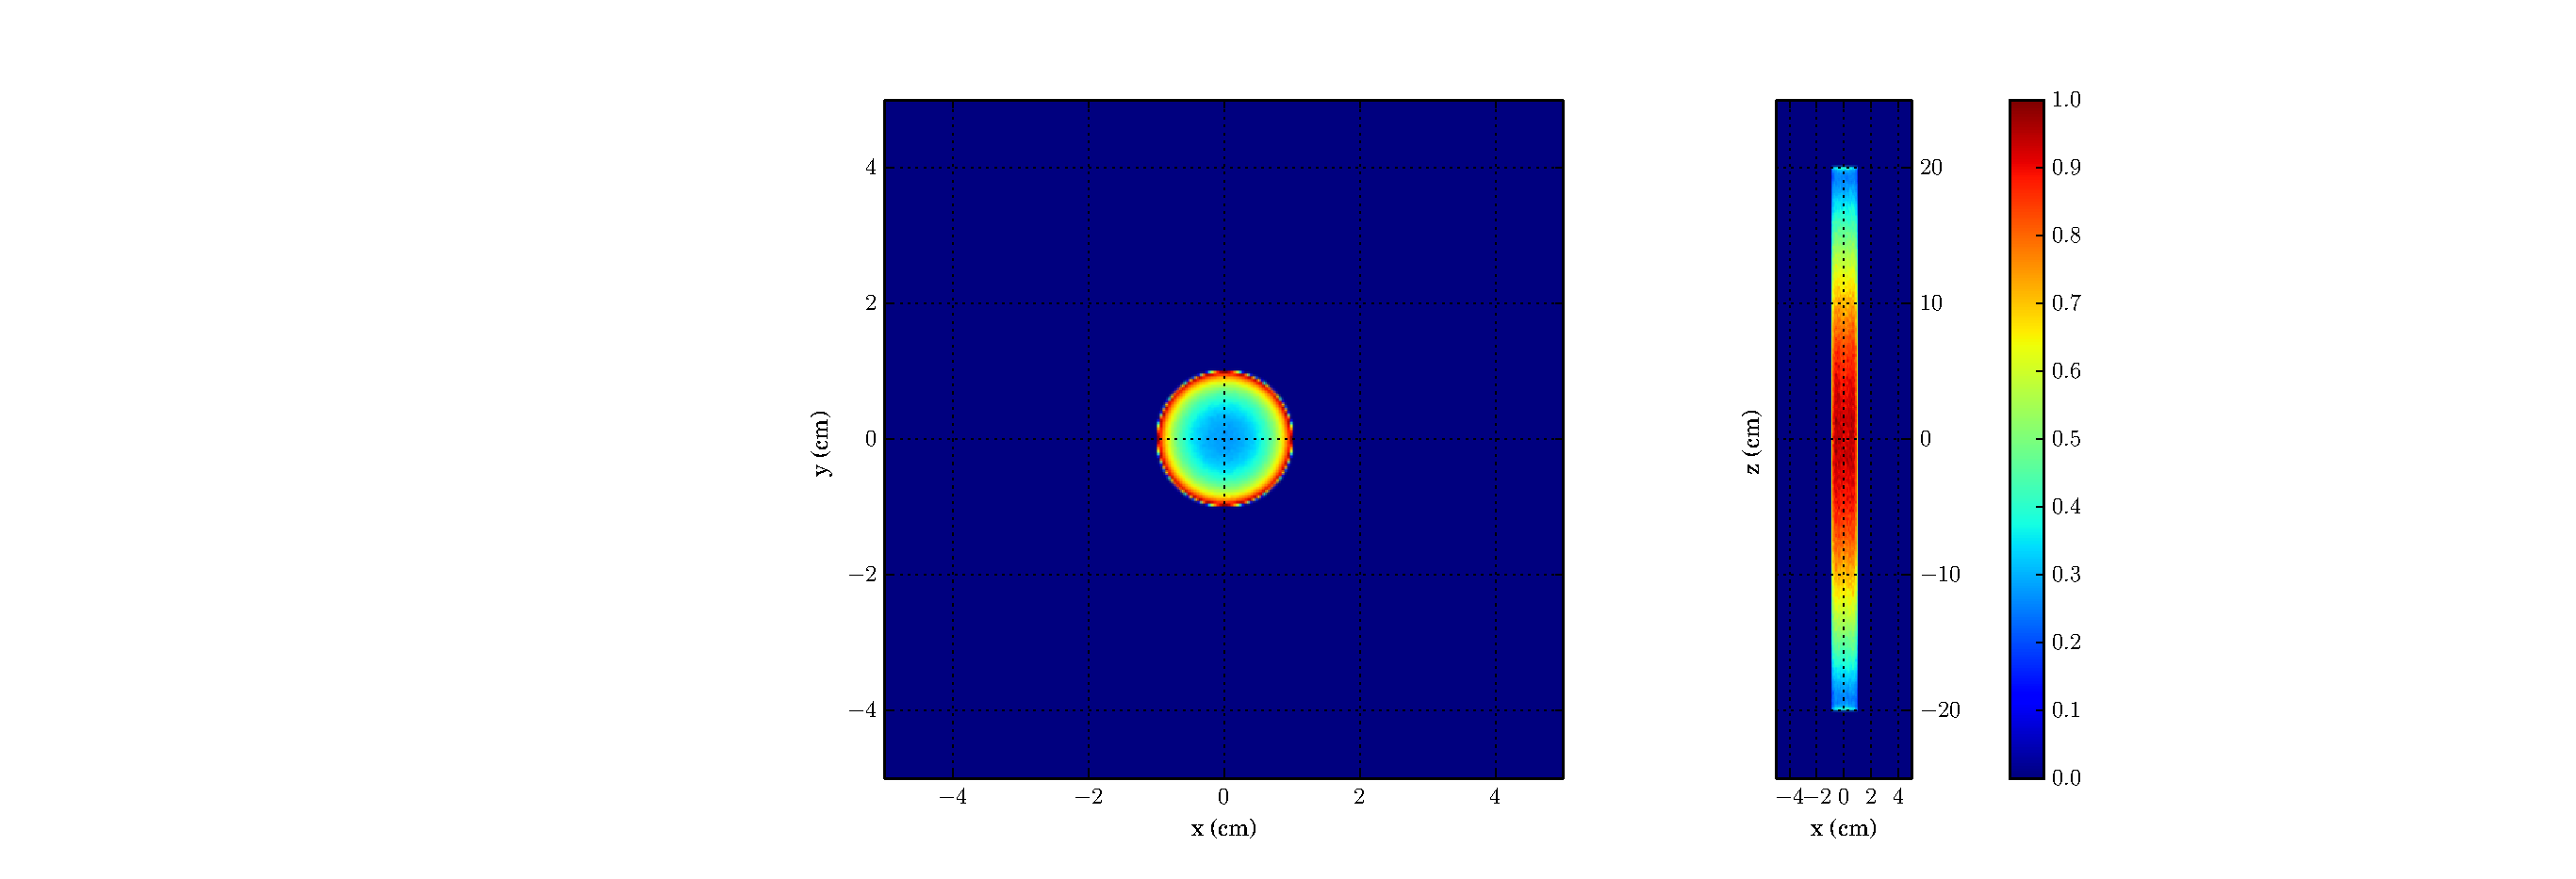
\includegraphics[width=\textwidth,trim= 10cm 0cm 6cm 0cm]{graphics/finalresults/pincell_fiss_serp-6.eps}
     \caption{Fission source distribution from Serpent 2.1.18 of a single UO$_2$ pin surrounded by a block of water  \label{serp_pincell_mesh} }
\end{figure}

\begin{figure}[h!] 
  \centering
    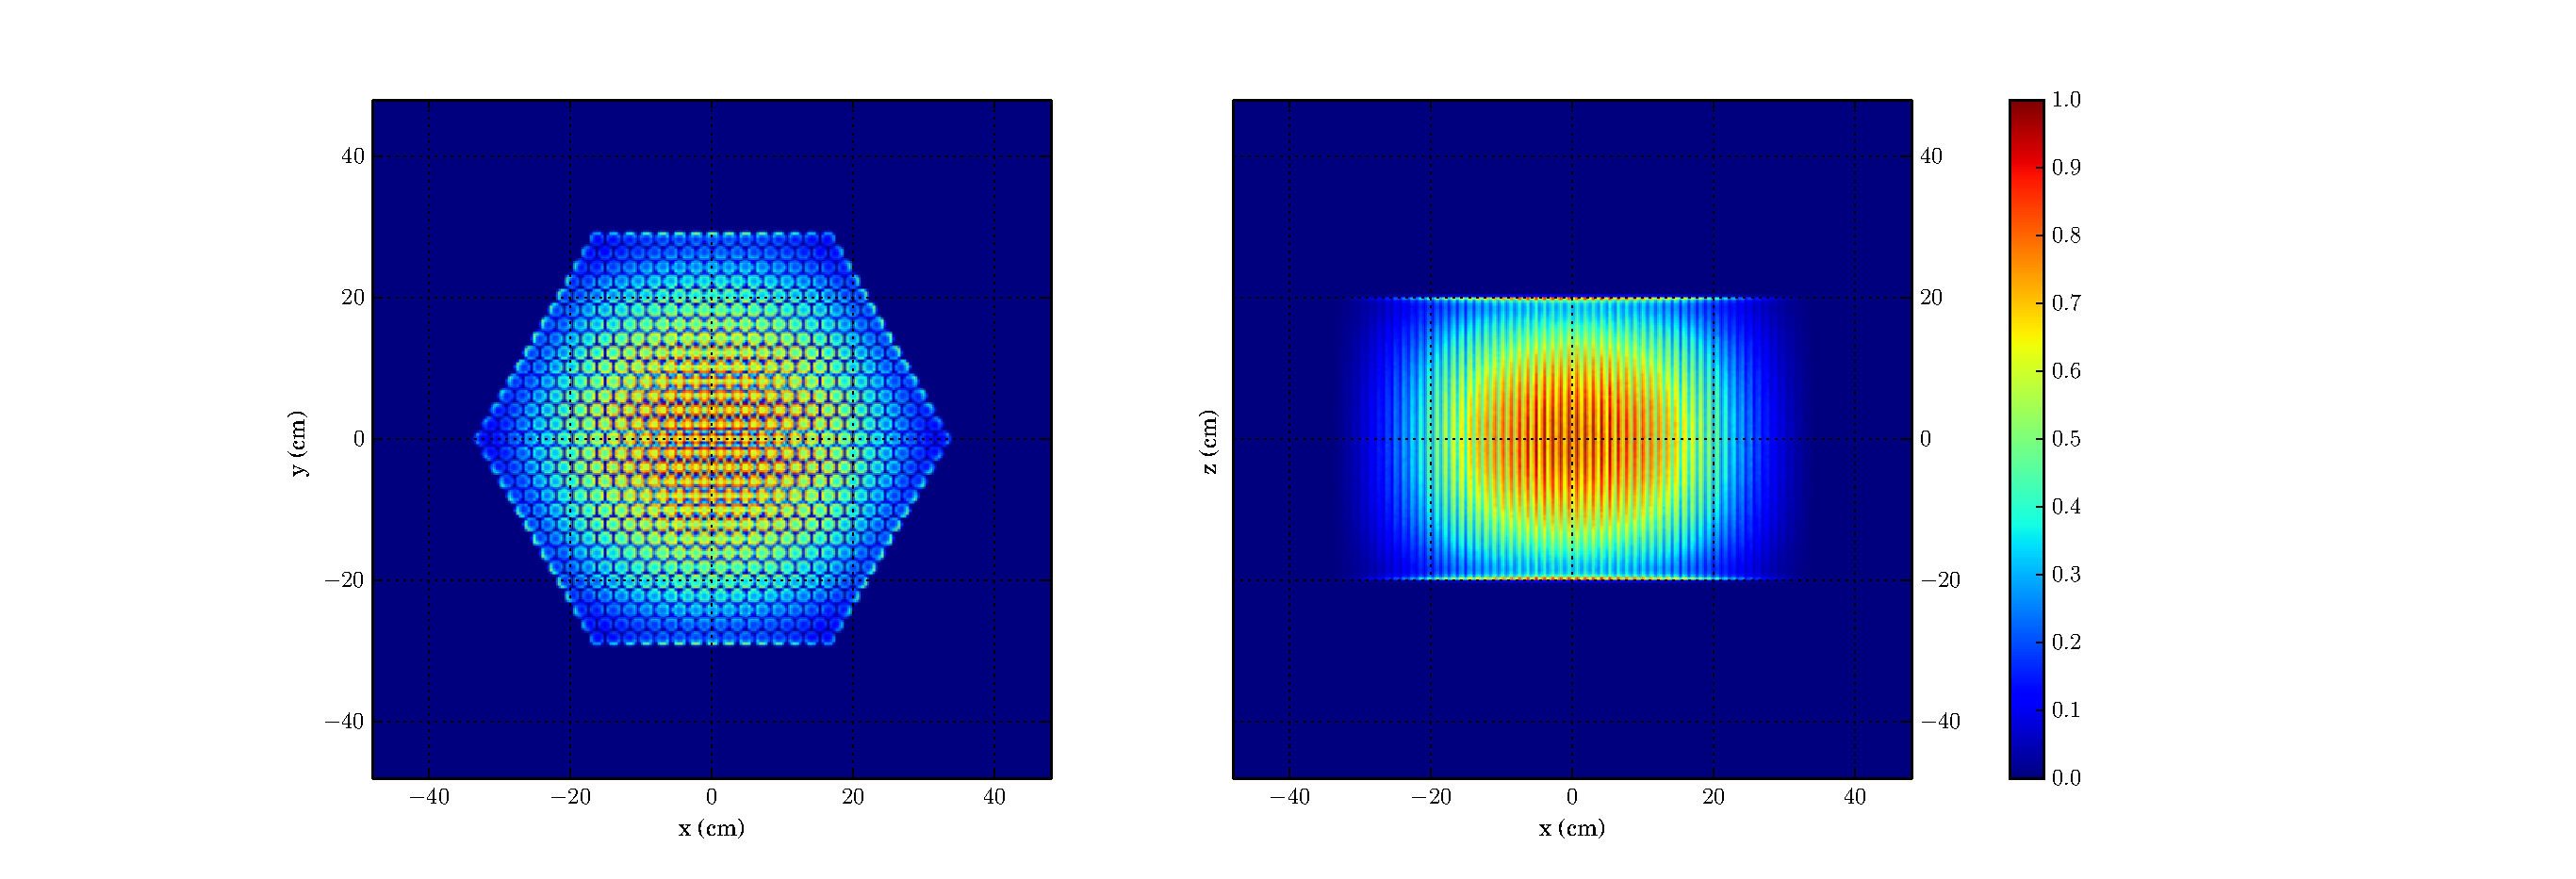
\includegraphics[width=\textwidth,trim= 4cm 0cm 6cm 0cm]{graphics/finalresults/assembly_fiss_serp-6.eps}
     \caption{Fission source distribution from Serpent 2.1.18 of a 15-sided hexagonal array of UO$_2$ pins in water. \label{serp_assembly_mesh} }
\end{figure}
